
%%% glcd_and_touchscreen_functions_for_velleman_VMA412.tex
%%%
%%%   Documentation for version 0.1rc1
%%%
%%%
%%% Copyright 2020 J.E.J. op den BRouw
%%%
%%% This work may be distributed and/or modified under the
%%% conditions of the LaTeX Project Public License, either version 1.3
%%% of this license or (at your option) any later version.
%%% The latest version of this license is in
%%%   http://www.latex-project.org/lppl.txt
%%% and version 1.3 or later is part of all distributions of LaTeX
%%% version 2005/12/01 or later.
%%%
%%% This work has the LPPL maintenance status `maintained'.
%%% 
%%% The Current Maintainer of this work is J.E.J. op den Brouw.


\documentclass[12pt]{article}

\usepackage{parskip}
\usepackage[charter]{mathdesign}
\usepackage{nimbusmono}
\usepackage[margin=1in]{geometry}
\usepackage{graphicx}
%\usepackage{tocloft}
%\setlength\cftsubsecnumwidth{3.5em}
%% Indexing words...
\usepackage[noautomatic]{imakeidx}
%% The index page is typeset...
\indexsetup{othercode=\footnotesize}
\makeindex[columns=2]
%\usepackage{showidx}
\newcommand{\ifunc}[1]{\index{\texttt{#1}}}


\usepackage{listings}

\usepackage{hyperref}

\lstset{
    language=C,
    basicstyle=\small\ttfamily,
    xleftmargin=1em
}


\author{Version 0.1rc1\\[2ex]Jesse op den Brouw\thanks{Please mail me at: \href{mailto:J.E.J.opdenBrouw@hhs.nl}{J.E.J.opdenBrouw@hhs.nl}}\\The Hague University of Applied Sciences\\(THUAS)}
\title{Graphic LCD and Touchscreen Functions for Velleman VMA412 with ILI9341 Controller used with a STM32F446 Nucleo Board}
\date{\today}


\begin{document}

\raggedbottom
\maketitle

\vfill
{\small\leftskip=1em\rightskip=1em
The Velleman VM412 is an Arduino Uno/Mega compatible 2.8" color Graphic LCD with 320x240 pixels controlled by an ILI9431 graphic controller. The ILI9431 is connected using an 8-bit 8080 interface to the board. More information can be found via \url{https://www.velleman.eu/products/view/?id=435582}. There are a number second sources for this board such as the Makerfactory 2.8" Touchscreen and the ELEGOO UNO R3 2.8 Inches TFT Touch Screen.

The library is written in C and consists of four driver files and one C test file.

Library functions include plotting a pixel, rectangles, circles, arcs, printing strings, rotating displays and filling an object, and reading X, Y and pressure values. It also has primitive console based printing functions.

The library uses 18-bit colors where each color has 6 bits used.

The library is tested using a STM32F446 Nucleo board and STMCubeIDE version 1.3.1.

The VMA412 has an SD-card socket. This library has \textbf{no} support for accessing SD-cards.

}
\vfill

\newpage

\tableofcontents


\newpage

\section{Software License}
This software is licensed with the BSD License:

\begin{lstlisting}[basicstyle=\footnotesize\ttfamily]
Software License Agreement (BSD License)

Copyright (c) 2020 Jesse op den Brouw.  All rights reserved.

Portions based on :
 Copyright (c) 2012 Adafruit Industries.  All rights reserved.

Redistribution and use in source and binary forms, with or without
modification, are permitted provided that the following conditions are met:

- Redistributions of source code must retain the above copyright notice,
  this list of conditions and the following disclaimer.
- Redistributions in binary form must reproduce the above copyright notice,
  this list of conditions and the following disclaimer in the documentation
  and/or other materials provided with the distribution.

THIS SOFTWARE IS PROVIDED BY THE COPYRIGHT HOLDERS AND CONTRIBUTORS "AS IS"
AND ANY EXPRESS OR IMPLIED WARRANTIES, INCLUDING, BUT NOT LIMITED TO, THE
IMPLIED WARRANTIES OF MERCHANTABILITY AND FITNESS FOR A PARTICULAR PURPOSE
ARE DISCLAIMED. IN NO EVENT SHALL THE COPYRIGHT HOLDER OR CONTRIBUTORS BE
LIABLE FOR ANY DIRECT, INDIRECT, INCIDENTAL, SPECIAL, EXEMPLARY, OR
CONSEQUENTIAL DAMAGES (INCLUDING, BUT NOT LIMITED TO, PROCUREMENT OF
SUBSTITUTE GOODS OR SERVICES; LOSS OF USE, DATA, OR PROFITS; OR BUSINESS
INTERRUPTION) HOWEVER CAUSED AND ON ANY THEORY OF LIABILITY, WHETHER IN
CONTRACT, STRICT LIABILITY, OR TORT (INCLUDING NEGLIGENCE OR OTHERWISE)
ARISING IN ANY WAY OUT OF THE USE OF THIS SOFTWARE, EVEN IF ADVISED OF THE
POSSIBILITY OF SUCH DAMAGE.
\end{lstlisting}


\section{Documentation License}
This documentation is licensed with the Latex Project Public License:

\begin{lstlisting}[basicstyle=\footnotesize\ttfamily,showspaces=false,showstringspaces=false]
Copyright 20205 J.E.J. op den BRouw

This work may be distributed and/or modified under the
conditions of the LaTeX Project Public License, either version 1.3
of this license or (at your option) any later version.
The latest version of this license is in
  http://www.latex-project.org/lppl.txt
and version 1.3 or later is part of all distributions of LaTeX
version 2005/12/01 or later.

This work has the LPPL maintenance status `maintained'.
 
The Current Maintainer of this work is J.E.J. op den Brouw.
\end{lstlisting}


\section{Mouting the VMA412}
The Velleman VM412 is an Arduino Uno/Mega compatible 2.8" color Touchscreen Graphic LCD with 320x240 pixels controlled by an ILI9431 graphic controller.
The VMA412 has an Arduino Uno compatible connection and can be connected to numerous STM32F Nucleo boards.
Place the VM412 board as instructed. See Figure~\ref{fig:1} for a visual inspection.

\begin{figure}[!ht]
\centering
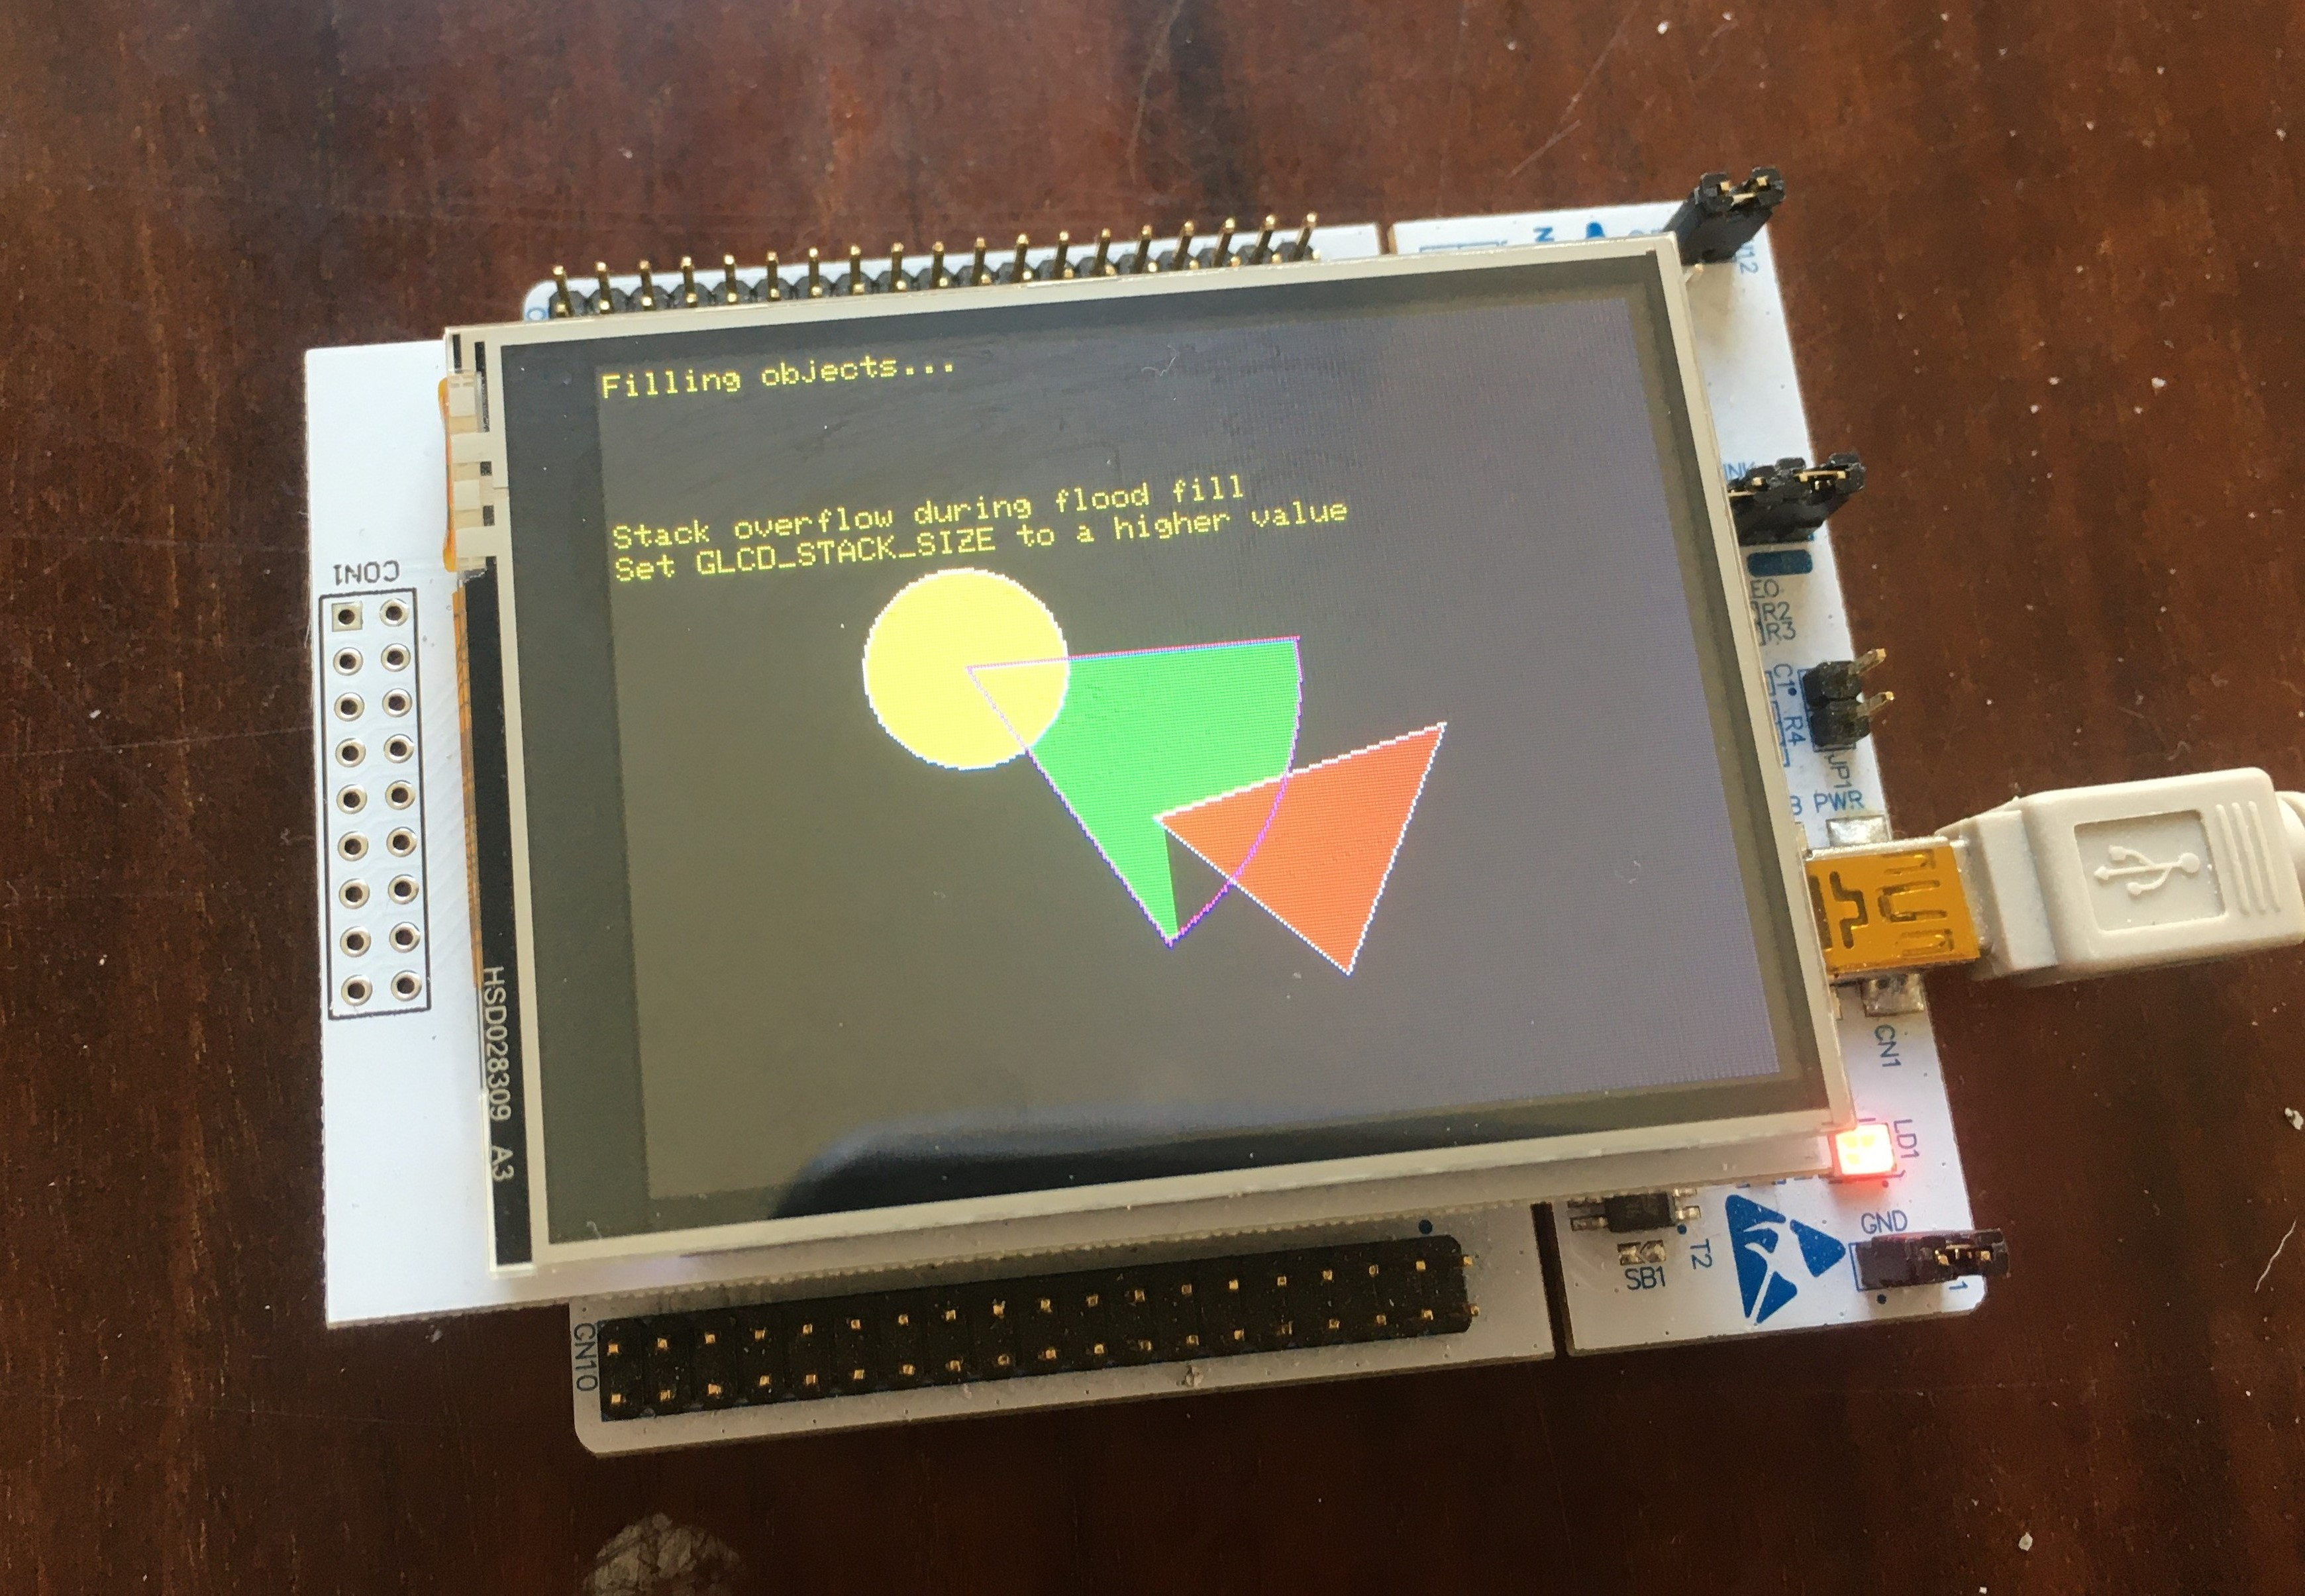
\includegraphics[width=0.7\textwidth]{glcd_demo}
\caption{Showing the VMA412 mounted on a STM32F446 Nucleo board.}
\label{fig:1}
\end{figure}


\section{Creating a project}
If you have downloaded the code from GitHub, then you already have all files needed. Just start STMCubeIDE and open the project. If you need to create a fresh project, make sure that you have selected the correct device. 
After creating a project, make sure that the five files are in the appropriate folders. These files are:

\begin{lstlisting}
glcd_ili9341_vma412.h   -- place in Core/Inc, definitions, typedefs etc
glcd_ili9341_vma412.c   -- place in Core/Src, functions to call
touchscreen_vma412.h    -- place in Core/Inc, definitions, typedefs etc
touchscreen_vma412.c    -- place in Core/Src, functions to call
main.c                  -- place in Core/Src, demo using functions
\end{lstlisting}


\section{Running the demo}
If you have set up your project just start compilation using \texttt{Project}$\rightarrow$\texttt{Build Project}. Then start the the demo using \texttt{Run}$\rightarrow$\texttt{Run}. The demo starts by asking you to touch one of four rectangles to start the GLCD demo, the touchscreen demo, the rotation demo or the character set demo, see Figure~\ref{fig:2}. At the end of the GLCD demo, there will be a list of running times for selected graphic functions as can be seen in Figure~\ref{fig:3}.

\begin{figure}[!ht]
\centering
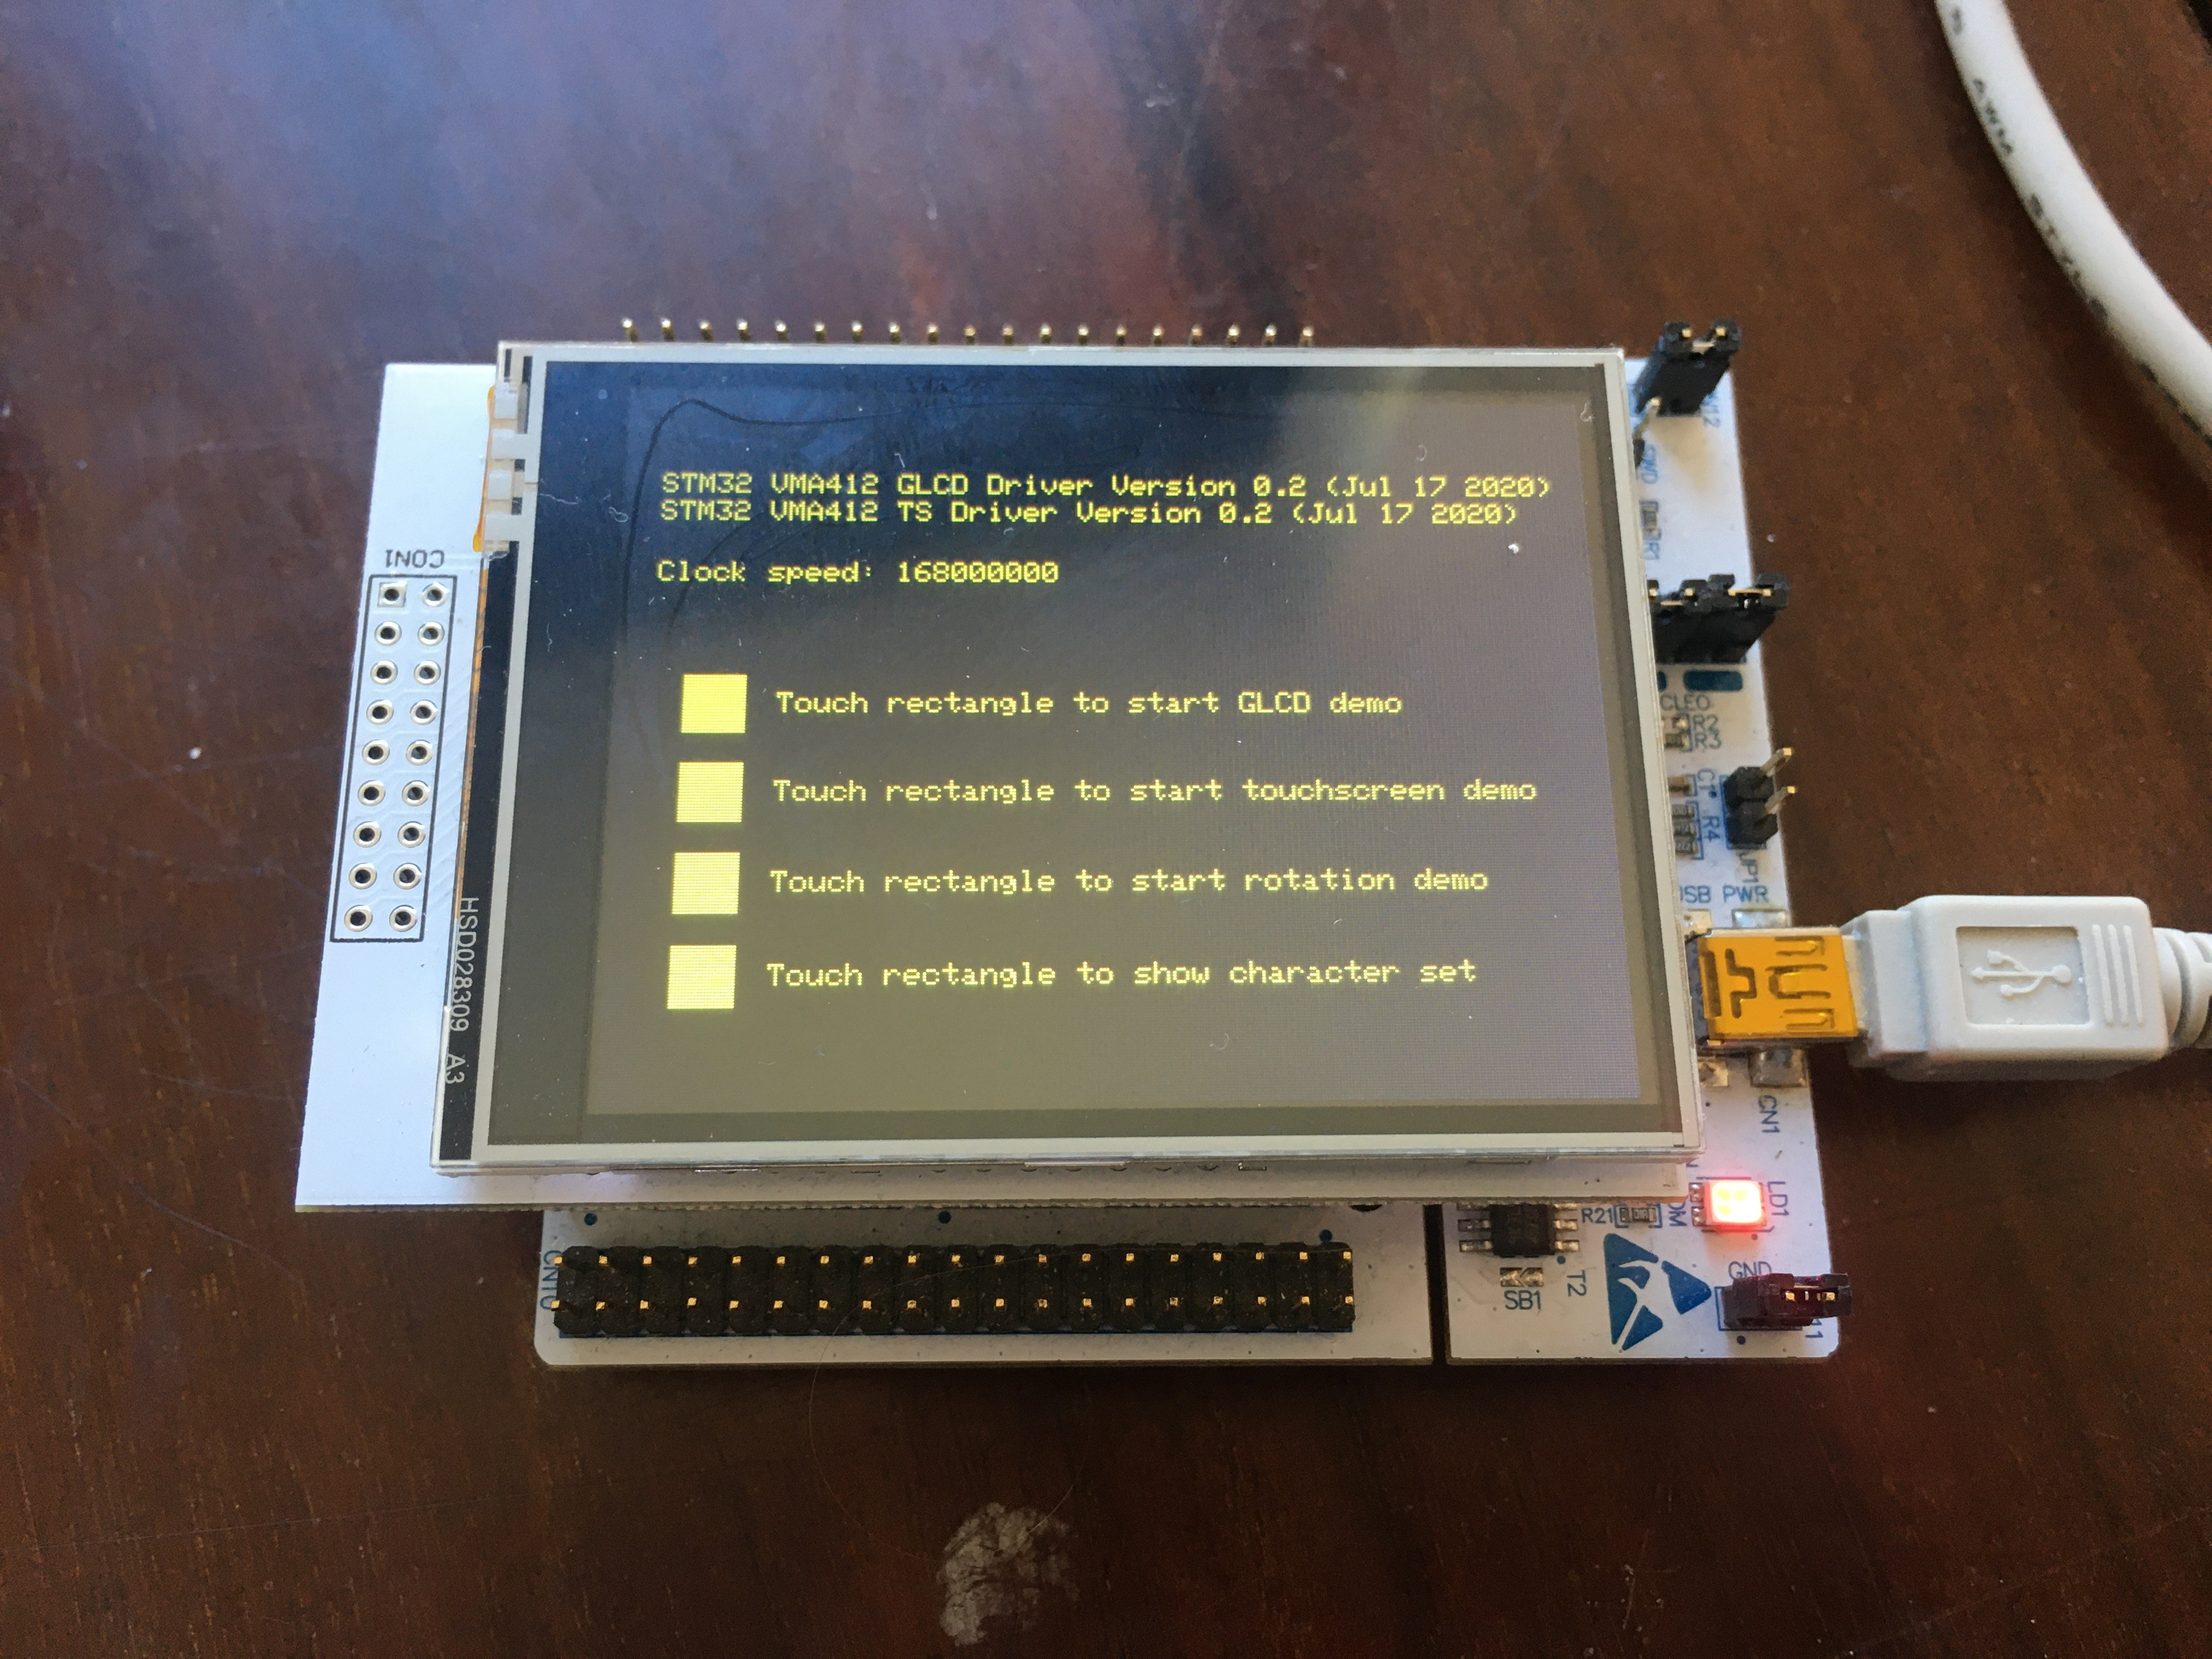
\includegraphics[width=0.7\textwidth]{start_demo}
\caption{Starting the demo.}
\label{fig:2}
\end{figure}

\begin{figure}[!ht]
\centering
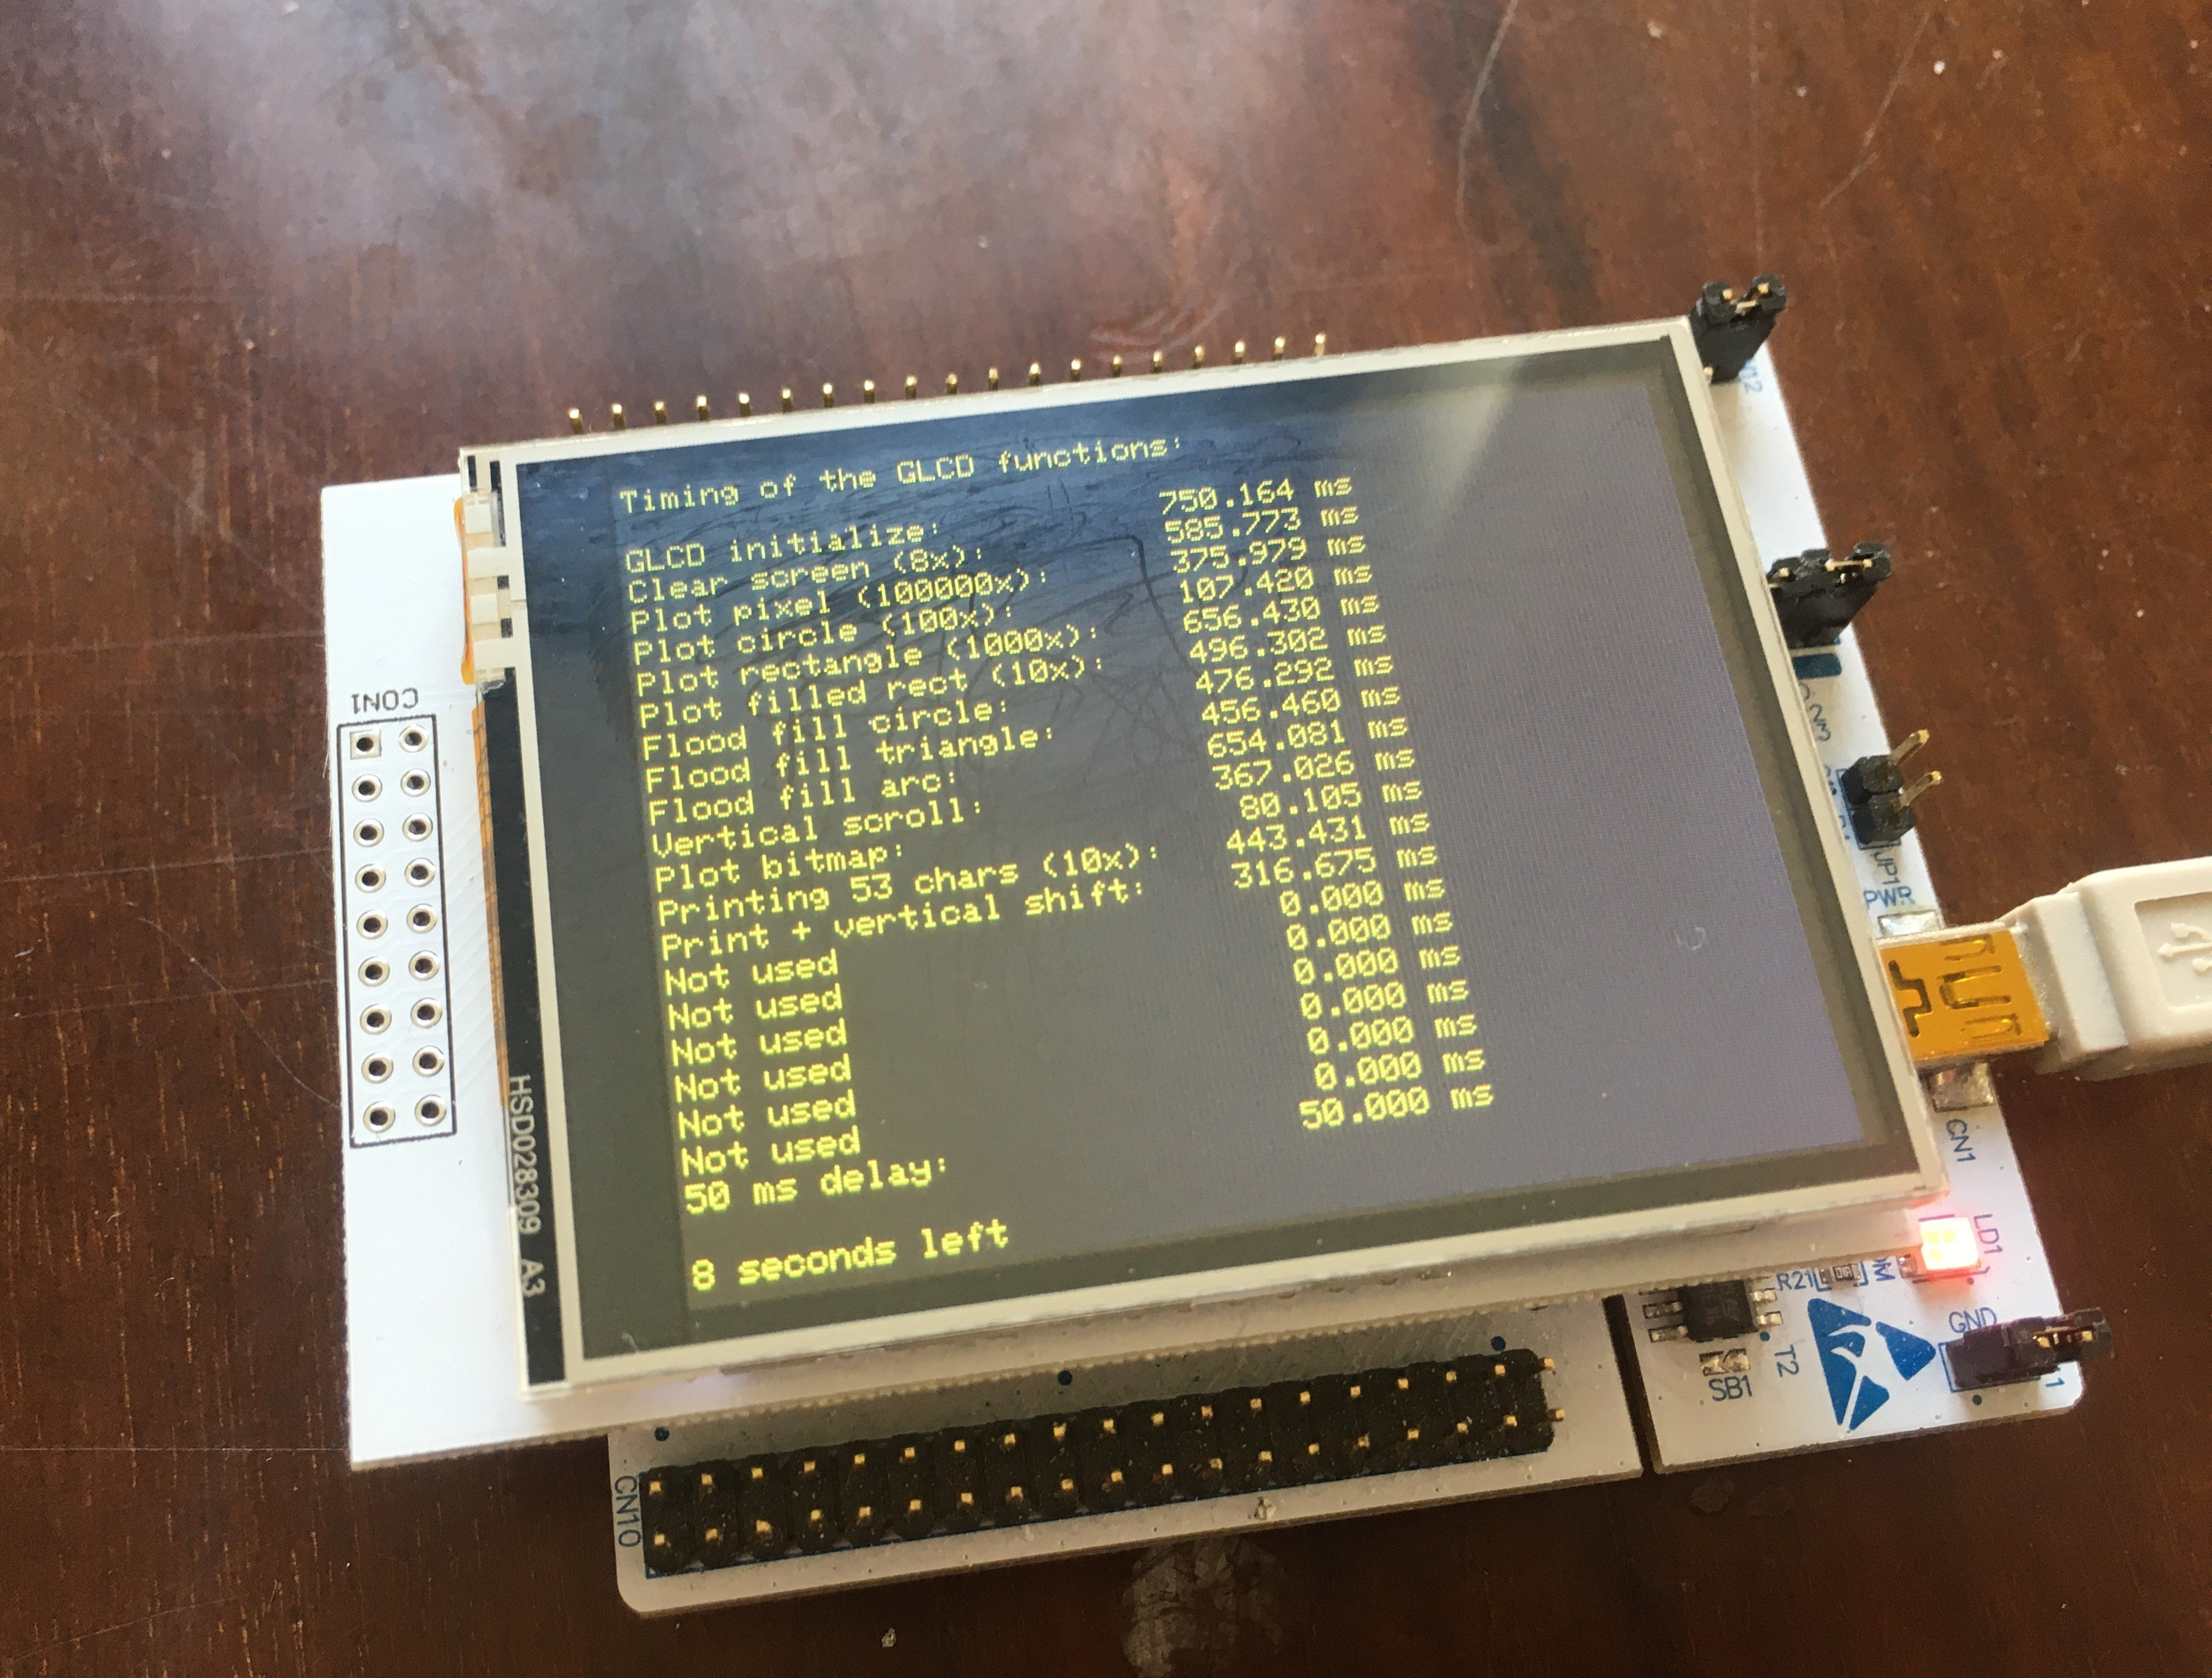
\includegraphics[width=0.7\textwidth]{times}
\caption{Displaying times for selected GLCD functions.}
\label{fig:3}
\end{figure}


\section{Color system}
\index{Color system}
The GLCD is set up to use the 18-bit color specification. This means that colors are specified with unsigned 32 bits. The specification is as follows:

Bits 31-24: ignored, should be kept at 0.\\
Bits 23-16: red -- only upper 6 bits are used\\
Bits 15-8: green -- only upper 6 bits are used\\
Bits 7-0: blue -- only upper 6 bits are used

Note: The 16 bit color specification in \textbf{NOT} supported, but they can be converted. See $\S$~\ref{sec:convertcolors}.

Please note that although 8 bits per color can be specified, only the upper 6 bits of each color are used, since the display uses 18 bits of color infomation. The lower 2 bits of each color are ignored. This means that color \lstinline|0x000000| and \lstinline|0x000001| are displayed the same, but are different in compares.

The color is specified using the the type \lstinline|glcd_color_t|. Note: don't ever change the type \lstinline|glcd_color_t|.

\subsection{Predefined colors}
\index{Predefined colors}
There are some predefines colors:

\begin{lstlisting}
#define GLCD_COLOR_BLACK   (0x000000)
#define GLCD_COLOR_BLUE    (0x0000ff)
#define GLCD_COLOR_GREEN   (0x00ff00)
#define GLCD_COLOR_CYAN    (0x00ffff)
#define GLCD_COLOR_RED     (0xff0000)
#define GLCD_COLOR_MAGENTA (0xff00ff)
#define GLCD_COLOR_YELLOW  (0xffff00)
#define GLCD_COLOR_WHITE   (0xffffff)

#define GLCD_COLOR_GREY50  (0x7f7f7f)

/* THUAS default color */
#define GLCD_COLOR_THUASGREEN ((158<<16)|(167<<8)|0)
\end{lstlisting}

\subsection{Using your own color}
To use your own color, please use the color type \lstinline|glcd_color_t|:

\begin{lstlisting}
glcd_color_t SkyBlue2 = (126<<16)|(192<<8)|238
\end{lstlisting}

as taken for the \LaTeX\ \lstinline|xcolor| package (\url{https://www.ctan.org/pkg/xcolor}).

Note: don't ever change the type \lstinline|glcd_color_t|.


\section{X and Y coordinates, display orientation}
\index{Coordinate system}\index{Display orientation}
The X and Y coordinates use type \lstinline|uint16_t| for their values. The display is set up in landscape where \lstinline|X| is between 0 and 319 and \lstinline|y| is between 0 and 239. Point (0,0) is in the upper left corner,
point (239,319) is in the lower right corner. The landscape orientation is with the SD-card socket to the right.
The display orientation can be changed, see $\S$~\ref{sec:rotdispl}.


\section{Graphic LCD}
\subsection{GLCD Initialization}
First you have to set up the clock system used by the STM32F microcontroller. If you use the external clock generator, make sure that the value of \lstinline|HSE_VALUE| is set to the correct frequency. In the case of the Nucleo board it is 8000000 (8 MHz). This value is defined in \lstinline|stm32f4xx_hal_conf.h| and \lstinline|system_stm32f4xx.c|.

If you use the internal HSI (\lstinline|HSIVALUE|), the frequency is 16 MHz by default. Best is to set up the clock speed to the maximum frequency allowed by the microcontroller.

Initialize the display by calling the \lstinline|glcd_init()| function. After calling that function the display is initialized and ready for use.

\subsubsection{Initialize display}
Note: call this function \textbf{after} the clock system is set up.

This function must be called after the clock system is set up and before using any other GLCD functions. The function prototype is:
\begin{lstlisting}
void glcd_init(void);
\end{lstlisting}

\subsection{Very low GLCD functions}

\subsubsection{Setting the write delay}
\ifunc{glcd\_set\_write\_pulse\_delay}
\textbf{Note:} use with care.\\
Sets the delay for write actions. There is no need to call this function as the correct timing is calculated according to the system clock speed after the clock system is set up, but you can tweak this value to get maximum performance. \lstinline|delay| must be greater than 0. The function prototype is:
\begin{lstlisting}
void glcd_set_write_pulse_delay(uint32_t delay);
\end{lstlisting}

\subsubsection{Setting the read delay}
\ifunc{glcd\_set\_read\_pulse\_delay}
\textbf{Note:} use with care.\\
Sets the delay for read actions. There is no need to call this function as the correct timing is calculated according to the system clock speed after the clock system is set up, but you can tweak this value to get maximum performance. \lstinline|delay| must be greater than 0. The function prototype is:

\begin{lstlisting}
void glcd_set_read_pulse_delay(uint32_t delay);
\end{lstlisting}

\subsection{GLCD low level functions}
\ifunc{glcd\_read\_terminate}
There are a number of low level functions. They are normally not needed.

\subsubsection{Reading data from the display}

Te read data from the display, use the function \lstinline|glcd_read_terminate|. Reading is explicitly terminated. The function prototype is:

\begin{lstlisting}
void glcd_read_terminate(uint16_t cmd,            // The command
                         uint16_t amount,         // Amount of data
                         glcd_buffer_t data[]);   // The buffer
\end{lstlisting}

Note: is you read pixel color information (scan line), the first \lstinline|uint16_t| of the buffer is useless information.

\subsubsection{Writing data to the display}
\ifunc{glcd\_write}
Writes data to the display, no explicit terminate. This means that multiple writes can be done in sequence.
\begin{lstlisting}
void glcd_write(uint16_t cmd,                     // The command
                uint16_t amount,                  // Amount of data
                const glcd_buffer_t data[]);      // The buffer
\end{lstlisting}

\subsubsection{Explicit terminating a write}
\ifunc{glcd\_terminate\_write}
Terminates a write:
\begin{lstlisting}
void gcld_terminate_write(void);
\end{lstlisting}

\subsubsection{Changing the buffer type}
\index{Changing buffer type}
\label{sec:changebuf}
The low level functions use an internal buffer. The buffer is of type \lstinline|glcd_buffer_t|. This normally set to an unsigned 16-bit size. This size can be changed:

Set to \lstinline|uint8_t| for minimal resources\\
Set to \lstinline|uint16_t| for best speed\\
Set to \lstinline|uint32_t| for maximum capacity (not recommended)
 
\subsection{GLCD high level commands}

\subsubsection{Delay}
\ifunc{glcd\_delay\_ms}
To delay your applications (in milliseconds), use :

\begin{lstlisting}
void glcd_delay_ms(uint32_t delay);
\end{lstlisting}

\subsubsection{Rotating the display}
\ifunc{glcd\_setrotation}
\label{sec:rotdispl}

To set the rotation of the display, use:
\begin{lstlisting}
void glcd_setrotation(glcd_rotation_t rot);
\end{lstlisting}

Where \lstinline|rot| is one of:

\begin{lstlisting}
GLCD_SCREEN_ROT0           // Standard landscape, default
GLCD_SCREEN_ROT90          // Rotate 90 degrees
GLCD_SCREEN_ROT180         // Rotate 180 degrees
GLCD_SCREEN_ROT270         // Rotate 270 degrees
\end{lstlisting}

Notes on rotation:

When you rotate the display, the current display contents are not deleted. You have to clear the display explicitly.

The default rotation is 0$^\circ$. The display is in landscape with the SD-card socket on the right of the display. A rotation of 90$^\circ$ sets the display is portrait mode with the SD-card socket at the bottom of the display. A rotation of 180$^\circ$ sets the display in landscape mode with the SD-card socket to the left of the Display. A rotation of 270$^\circ$ set the display in portrait mode with the SD-card socket at the top of the display.

To be compatible with Arduino-based software, set the rotation to 90$^\circ$.

Note: the touchscreen is \textbf{not} rotated. The touchscreen functions are setup for the standard rotation of 0$^\circ$. How to handle the touchscreen in case of rotated displays, see $\S$~\ref{sec:rottouch}.

\subsubsection{Clear the display}
\ifunc{glcd\_cls}

To clear the display with a color, use:
\begin{lstlisting}
void glcd_cls(glcd_color_t color);
\end{lstlisting}

\subsubsection{Plot a pixel}
\ifunc{glcd\_plotpixel}
To plot a pixel, use:
\begin{lstlisting}
void glcd_plotpixel(uint16_t x,           // x coordinate
                    uint16_t y,           // y coordinate
                    glcd_color_t color);  // color
\end{lstlisting}

Note: if \lstinline|x| is greater that the width of the display minus 1, the pixel is not plotted.\\
Note: if \lstinline|y| is greater that the height of the display, minus 1, the pixel is not plotted.\\

\subsubsection{Read a pixel}
\ifunc{glcd\_readpixel}
To read a pixel (getting color information) in \lstinline|glcd_color_t| use:

\begin{lstlisting}
glcd_color_t glcd_readpixel(uint16_t x,   // x coordinate
                            uint16_t y);  // y coordinate
\end{lstlisting}

Note: if \lstinline|x| is greater that the width of the display minus 1, the returned color is undefined.\\
Note: if \lstinline|y| is greater that the height of the display, minus 1, the returned color is undefined.\\

\subsubsection{Plot a horizontal line}
\ifunc{glcd\_plothorizontalline}
To plot a horizontal line (fast), use:
\begin{lstlisting}
void glcd_plothorizontalline(uint16_t x,           // x coordinate
                             uint16_t y,           // y coordinate
                             uint16_t w,           // width
                             glcd_color_t color);  // color
\end{lstlisting}

Note: if \lstinline|x+w| is greater than the width of the display minus 1, the pixels in excess are not plotted.

\subsubsection{Plot a vertical line}
\ifunc{glcd\_plotverticalline}
To plot a vertical line (fast), use:
\begin{lstlisting}
void glcd_plotverticalline(uint16_t x              // x coordinate
                           uint16_t y,             // y coordinate
                           uint16_t h,             // height
                           glcd_color_t color);    // color
\end{lstlisting}
Note: if \lstinline|y+h| is greater than the height of the display minus 1, the pixels in excess are not plotted.

\subsubsection{Plot a line with any angle and length}
\ifunc{glcd\_plotline}
To plot a line with any angle and length, use:
\begin{lstlisting}
void glcd_plotline(uint16_t x0,            // x start point
                   uint16_t y0,            // y start point
                   uint16_t x1,            // x end point
                   uint16_t y1,            // y end point
                   glcd_color_t color);    // color
\end{lstlisting}

Note: the part of the line that is exceeding the dimensions of the display are not plotted.

\subsubsection{Plot a character using buildin font}
\ifunc{glcd\_plotchar}
To plot a character using the buildin font (5x8), use:
\begin{lstlisting}
void glcd_plotchar(uint16_t x,             // x coordinate
                   uint16_t y,             // y coordinate
                   uint8_t c,              // character (0-255)
                   glcd_color_t color,     // color
                   glcd_color_t bg);       // background color
\end{lstlisting}

Note: character is one of 0 -- 255 (no special C treatment)\\
Note: if \lstinline|color| is equal to \lstinline|bg| then pixels having background color are not printed!

\subsubsection{Plot a string using buildin font}
\ifunc{glcd\_plotstring}
To plot a string using the buildin font, use:
\begin{lstlisting}
void glcd_plotstring(uint16_t x,                  // x coordinate
                     uint16_t y,                  // y coordinate
                     char str[],                  // the string
                     glcd_color_t color,          // color
                     glcd_color_t bg,             // background color
                     glcd_spacing_t spacing);     // spacing
\end{lstlisting}

Note: a \lstinline|\0| terminates a string (as in C). This means that buildin character 0 cannot be printed\\
Note: if \lstinline|color| is equal to \lstinline|bg| then pixels having background color are not printed\\
Note: \lstinline|spacing| is one of:
\begin{lstlisting}
GLCD_STRING_CONDENSED  // zero pixels apart
GLCD_STRING_NORMAL     // one pixel apart
GLCD_STRING_WIDE       // two pixels apart
\end{lstlisting}

\subsubsection{Plot a rectangle}
\ifunc{glcd\_plotrect}
To plot a rectangle, use:
\begin{lstlisting}
void glcd_plotrect(uint16_t x,             // x coordinate
                   uint16_t y,             // y coordinate
                   uint16_t w,             // width
                   uint16_t h,             // height
                   glcd_color_t color);    // color
\end{lstlisting}

Note: \lstinline|x| and \lstinline|y| specify the upper left corner.

\subsubsection{Plot a filled rectangle}
\ifunc{glcd\_plotrectfill}
To plot a filled rectangle, use:
\begin{lstlisting}
void glcd_plotrectfill(uint16_t x,            // x coordinate
                       uint16_t y,            // y coordinate
                       uint16_t w,            // width
                       uint16_t h,            // height
                       glcd_color_t color);   // color
\end{lstlisting}

Note: \lstinline|x| and \lstinline|y| specify the upper left corner.

\subsubsection{Plot a rectangle with rounded corners}
\ifunc{glcd\_plotrectrounded}
To plot a rectangle with rounded corners, use:

\begin{lstlisting}
void glcd_plotrectrounded(uint16_t x,           // x coordinate
                          uint16_t y,           // y coordinate
                          uint16_t w,           // width
                          uint16_t h,           // height
                          uint16_t r,           // radius
                          glcd_color_t color);  // color
\end{lstlisting}

Note: \lstinline|x| and \lstinline|y| specify the upper left corner as plotted with \lstinline|glcd_plotrect|.

\subsubsection{Plot a filled rectangle with rounded corners}
\ifunc{glcd\_plotrectroundedfill}
To plot a filled rectangle with rounded corners, use:

\begin{lstlisting}
void glcd_plotrectroundedfill(uint16_t x,           // x coordinate
                              uint16_t y,           // y coordinate
                              uint16_t w,           // width
                              uint16_t h,           // height
                              uint16_t r,           // radius
                              glcd_color_t color);  // color
\end{lstlisting}

Note: \lstinline|x| and \lstinline|y| specify the upper left corner as plotted with \lstinline|glcd_plotrect|.

\subsubsection{Plot a circle}
\ifunc{glcd\_plotcircle}
To plot a circle, use:
\begin{lstlisting}
void glcd_plotcircle(uint16_t x0,             // center x coordinate
                     uint16_t y0,             // center y coordinate
                     uint16_t r,              // radius
                     glcd_color_t color);     // color
\end{lstlisting}

\subsubsection{Plot a filled circle}
\ifunc{glcd\_plotcirclefill}
To plot a filled circle, use:
\begin{lstlisting}
void glcd_plotcirclefill(uint16_t x0,             // center x coordinate
                         uint16_t y0,             // center y coordinate
                         uint16_t r,              // radius
                         glcd_color_t color);     // color
\end{lstlisting}

\subsubsection{Plot quarters of a circle}
\ifunc{glcd\_plotcirclequarter}
To plot quarters of a circle, use:
\begin{lstlisting}
void glcd_plotcirclequarter(uint16_t x0,               -- center x
                            uint16_t y0,               -- center y
                            uint16_t r,                -- radius
                            glcd_corner_t cornername,  -- corners
                            glcd_color_t color);       -- color
\end{lstlisting}

Note: this function doesn't plot the start and end points\\
Note: \lstinline|cornername| is one of or a composition of: 
\lstinline|GLCD_CORNER_UPPER_LEFT|,\\ \lstinline|GLCD_CORNER_UPPER_RIGHT|, \lstinline|GLCD_CORNER_LOWER_RIGHT| and \lstinline|GLCD_CORNER_LOWER_LEFT|

\subsubsection{Plot and fill left and/or right halves of a circle}
\ifunc{glcd\_plotcirclehalffill}
To plot and fill left and/or right halves of a circle, use:

\begin{lstlisting}
void glcd_plotcirclehalffill(uint16_t x0,                 -- center x
                             uint16_t y0,                 -- center y
                             uint16_t r,                  -- radius
                             glcd_cornerhalves_t corners, -- see notes
                             int16_t delta,               -- see notes
                             glcd_color_t color);         -- color
\end{lstlisting}

Notes \lstinline|delta| is the squeeze factor, positive squeezes left/right, negative squeezes top/bottom, 0 for plain circle.\\
Note: \lstinline|corners| is one of \lstinline|GLCD_CORNER_LEFT_HALF|, \lstinline|GLCD_CORNER_RIGHT_HALF| and\\ \lstinline|GLCD_CORNER_BOTH|.\\
Note: doesn't plot the outer top-to-bottom vertical line. 


\subsubsection{Plot an arc}
\ifunc{glcd\_plotarc}
To plot an arc, use:
\begin{lstlisting}
void glcd_plotarc(uint16_t xc,                // center x coordinate
                  uint16_t yc,                // center y coordinate
                  uint16_t r,                 // radius
                  float start,                // start angle in degrees
                  float stop,                 // stop angle in degrees
                  glcd_color_t color);        // color
\end{lstlisting}

Note: this function is only available if \lstinline|GLCD_USE_ARC| is defined.\\
Note: this function uses \lstinline|sinf| and \lstinline|cosf| math functions, using the onboard FPU.

\subsubsection{Plot a triangle}
\ifunc{glcd\_plottriangle}
To plot a triangle, use:

\begin{lstlisting}
void glcd_plottriangle(uint16_t x1,          // start x
                       uint16_t y1,          // start y
                       uint16_t x2,          // second x
                       uint16_t y2,          // second y
                       uint16_t x3,          // last x
                       uint16_t y3,          // last y
                       glcd_color_t color);  // color
\end{lstlisting}


\subsubsection{Plot a 2-color bitmap}
\ifunc{glcd\_plotbitmap}
To plot a 2-color bitmap, use:
\begin{lstlisting}
void glcd_plotbitmap(uint16_t x,              // x coordinate
                     uint16_t y,              // y coordinate
                     const uint8_t bitmap[],  // the bitmap, see note
                     uint16_t w,              // width
                     uint16_t h,              // height
                     glcd_color_t color,      // color
                     glcd_color_t bg);        // background color
\end{lstlisting}

Note: \lstinline|bitmap| consists of bytes (\lstinline|uint8_t|). A 1 in a byte is converted to \lstinline|color|, a 0 in a byte is converted to \lstinline|bg|.

Note: you will get compiler warnings if your bitmap is in RAM, because \lstinline|bitmap| is qualified as \lstinline|const|.

Note: if you need to convert your image to a 2-bit color bitmap, have a look at \url{https://lvgl.io/tools/imageconverter}.

\subsubsection{Plot a 256-color indexed bitmap}
\ifunc{glcd\_plotbitmap8bpp}
To plot a 256-color indexed bitmap, use:
\begin{lstlisting}
void glcd_plotbitmap8bpp(uint16_t x,               // x start point
                         uint16_t y,               // y start point
                         uint16_t w,               // width
                         uint16_t h,               // height
                         const uint8_t *pic,       // start of image
                         const uint8_t *palette);  // start of palette
\end{lstlisting}

Note: each pixel is specified with a byte (\lstinline|uint8_t|). This is an index into the palette.\\
Note: each color is specified with a 32-bit RGB color specification. This means that each color takes up four bytes and the total palette size is 1024 bytes. The byte order for each indexed color is as follows: first byte is red, second byte is green, third byte is blue, fourth byte is not used.\\
Note: is \lstinline|palette| is equal to \lstinline|NULL| then the palette is at the start of the image and the image bytes follow the palette.

Note: you will get compiler warnings if your bitmap is in RAM, because \lstinline|bitmap| is qualified as \lstinline|const|.

Note: if you need to convert your image to a 256-color indexed image, have a look at \url{https://lvgl.io/tools/imageconverter}.

\subsubsection{Display inversion}
\ifunc{glcd\_inversion}
Sets the display inversion (or not):
\begin{lstlisting}
void glcd_inversion(glcd_display_inversion_t what);
\end{lstlisting}

Note: \lstinline|what| is one of:
\begin{lstlisting}
GLCD_DISPLAY_INVERSION_OFF
GLCD_DISPLAY_INVERSION_ON
\end{lstlisting}

\subsubsection{Display idle}
\ifunc{glcd\_idle}
Set the display to idle (or not):
\begin{lstlisting}
void glcd_idle(glcd_display_idle_t what);
\end{lstlisting}

Note: \lstinline|what| is one of:

\begin{lstlisting}
GLCD_DISPLAY_IDLE_OFF
GLCD_DISPLAY_IDLE_ON
\end{lstlisting}

\subsubsection{Display on or off}
\ifunc{glcd\_display}
Sets the display on or off:
\begin{lstlisting}
void glcd_display(glcd_display_t what);
\end{lstlisting}

Note: \lstinline|what| is one of

\begin{lstlisting}
GLCD_DISPLAY_OFF
GLCD_DISPLAY_ON
\end{lstlisting}

\subsubsection{Flood fill an object}
\ifunc{glcd\_floodfill}
Flood fill an object using a software stack based approach:
\begin{lstlisting}
void glcd_floodfill(uint16_t xs,                 // x start point
                    uint16_t ys,                 // y start point
                    glcd_color_t fillColor,      // color for pixel == 1
                    glcd_color_t defaultColor);  // color for pixel == 0
\end{lstlisting}

Note: this function is only available if \lstinline|GLCD_USE_FLOOD_FILL| is defined.\\
Note: set \lstinline|GLCD_STACK_SIZE| to an appropiate value.\\
Note: if you have problems filling an object increase the value of \lstinline|GLCD_STACK_SIZE|.\\
Note: the stack uses unsigned 32-bit entries so the complete stack uses \lstinline|GLCD_STACK_SIZE|*4 bytes of RAM.

\subsubsection{Scroll the display vertical upwards}
\ifunc{glcd\_scrollvertical}
To scroll the display vertical a number of lines, use:
\begin{lstlisting}
void glcd_scrollvertical(uint16_t lines);   // lines to scroll upwards
\end{lstlisting}

Note: this is a software based scroll, could be slow. The lines are scrolled upwards off the display (no rotation), and the vacant lines are left untouched.

\subsubsection{Console based character printing}
\ifunc{glcd\_putchar}
\label{sec:consolebasedcharacterprinting}
To use a simple console based character printing, use:
\begin{lstlisting}
void glcd_putchar(char c);
\end{lstlisting}

Note: characters are printed in yellow, background is black.\\
Note: \lstinline|\f| (form feed) clears the display.\\
Note: \lstinline|\n| returns and goes to the next line, may cause a vertical shift.\\
Note: \lstinline|\r| return to the beginning of the line.\\
Note: \lstinline|\b| erases last character and goes one character back (ultimate to the beginning of the line).\\
Note: \lstinline|\t| creates tab stops at 8 character intervals\\Note: all other characters are printed using the internal font.\\
Note: if a character ``falls off'' the display, line wrap will be used, may cause a vertical shift.\\
Note: this function is aware of the current display rotation.

\subsubsection{Console based string printing}
\ifunc{glcd\_puts}
To use a simple console based string printing use:
\begin{lstlisting}
void glcd_puts(char str[]);
\end{lstlisting}

Note: \lstinline|str| is terminated with \lstinline|\0| (as in C).\\
Note: see $\S$\ref{sec:consolebasedcharacterprinting} for character handling.\\
Note: if \lstinline|str| equals \lstinline|NULL|, then \lstinline|(null)| is printed.

\subsubsection{Get the current display width}
\ifunc{glcd\_getwidth}
To get the current display width, use:

\begin{lstlisting}
uint16_t glcd_getwidth(void);
\end{lstlisting}

\subsubsection{Get the current display height}
\ifunc{glcd\_getheight}
To get the current display height, use:
\begin{lstlisting}
uint16_t glcd_getheight(void);
\end{lstlisting}

\subsubsection{Converting 16 bit colors}
\ifunc{glcd\_convertcolor}
\label{sec:convertcolors}
To convert 16 bit standard colors to 24-bit colors, use:

\begin{lstlisting}
glcd_color_t glcd_convertcolor(uint16_t color16)
\end{lstlisting}

Note: 16 bit colors are composed of 5 bit red (bits 11 -- 15), 6 bit green (bits 5 -- 10) and 5 bit blue (bits 0 -- 4).\\
Note: although the returned color is specified as a 24-bit value, only 65536 different colors can be composed using 16-bit colors.

\subsection{GLCD Tayloring}
\index{GLCD tayloring}
There are a number of \lstinline|#define|'s that can be manipulated to taylor the GLCD functions to your needs. They can be found in \lstinline|glcd_ili9341_vma412.h|:

\begin{lstlisting}
#define GLCD_USE_FLOOD_FILL
#define GLCD_STACK_SIZE (2000)
#define GLCD_USE_FLOOD_FILL_PRINT_IF_STACK_OVERFLOW
#define GLCD_USE_ARC
#define GLCD_CHARCTERS_IN_RAM
#define GLCD_HAVE_THUAS_BITMAPS

#define GLCD_WIDTH (320)
#define GLCD_HEIGHT (240)
\end{lstlisting}

Define \lstinline|GLCD_USE_FLOOD_FILL| if you need to (flood) fill objects, undefine to save ROM  and RAM resources. If you use flood fill, set the stack size \lstinline|GLCD_STACK_SIZE| to an appropriate size. While testing or debugging, define \lstinline|GLCD_USE_FLOOD_FILL_PRINT_IF_STACK_OVERFLOW|. This will print warning messages if there is a stack overflow when filling objects. Undefine if you are sure there will be no stack overflow. Define \lstinline|GLCD_USE_ARC| if you need to plot arcs, undefine to save ROM resources. Plotting arcs use the onboard FPU for sine and cosine calculations. Define \lstinline|GLCD_CHARACTERS_IN_RAM| to place the character table in RAM. This way you can change the view of a character by changing the bit patterns (but of course is uses extra RAM). Define \lstinline|GLCD_HAVE_THUAS_BITMAPS| if you need the buildin THUAS logos (you probably won't need them).

Leave \lstinline|GLCD_WIDTH| and \lstinline|GLCD_HEIGHT| to their respective values.

The GLCD functions use an internal buffer. The size of the buffer elements are set to the type \lstinline|glcd_buffer_t|. This is normally set to unsigned 16-bit. The buffer length is set to \lstinline|GLCD_WIDTH|*3+1.

The size of the buffer elements can be changed, see~\ref{sec:changebuf}.

\begin{lstlisting}
typedef uint16_t glcd_buffer_t;
\end{lstlisting}

Set to \lstinline|uint8_t| for smallest RAM footprint, but causes extra CPU time. Set to \lstinline|uint16_t| for fastest processing, but wastes unused RAM. There is no speed gain when setting to \lstinline|uint32_t|. It just wastes resources.

\section{Touchscreen}
\subsection{Touchscreen Initialization}
Before using any of the touchscreen functions, you have to initialize the touchscreen. Reading the X and Y coordinates of the pressed touchscreen point needs one of the onboard ADC's. The function \lstinline|touchscreen_init| initializes the selected ADC. Please note that the selected ADC must be dedicated to the touchscreen functions, since the ADC is setup only once. Sharing the ADC with other functions is not recommended.

Please note that the ADC is setup for 10-bit conversions so the values returned are from 0 to 1023 (inclusive).

\subsection{Touchscreen low level functions}

\subsubsection{Set the ADC speed}
\ifunc{touchscreen\_setadcspeed}
\label{sec:setadcspeed}
To set the ADC speed (for all ADCs), use:

\begin{lstlisting}
void touchscreen_setadcspeed(uint32_t speed);
\end{lstlisting}

Note: \lstinline|speed| is one of 0 (divide system clock by 2), 1 (divide system clock by 4), 2 (divide system clock by 6) or 3 (divide system clock by 8). See $\S$~\ref{sec:touchinit}.\\
Note: call this function \textbf{after} the touchscreen is initialized.\\
Note: this speed will be set for all ADCs.

\subsubsection{Read raw X position}
\ifunc{touchscreen\_readrawx}
To read the current raw X position, use:

\begin{lstlisting}
uint32_t touchscreen_readrawx(void);
\end{lstlisting}

Note: this value is only of interest if the touchscreen is pressed\\
Note: returns the raw X position from the touchscreen. This value is an indication of where the touchscreen is pressed. It is not the actual X position as can be used with the GLCD functions. You need to map the raw X position.

\subsubsection{Read raw Y position}
\ifunc{touchscreen\_readrawy}
To read the current raw y position, use:

\begin{lstlisting}
uint32_t touchscreen_readrawy(void);
\end{lstlisting}

Note: this value is only of interest if the touchscreen is pressed\\
Note: returns the raw Y position from the touchscreen. This value is an indication of where the touchscreen is pressed. It is not the actual Y position as can be used with the GLCD functions. You need to map the raw Y position.

\subsubsection{Read raw pressure}
\ifunc{touchscreen\_pressure}
To read the raw pressure, use:

\begin{lstlisting}
uint32_t touchscreen_pressure(void);
\end{lstlisting}

Note: if the touchscreen is \textbf{not} pressed this functions returns a small number, typically 0. Any other values means that the touchscreen is pressed.

\subsubsection{Mapping the raw X and Y values to display coordinates}
\ifunc{touchscreen\_map}
To map raw X and Y values to display coordinates, use:

\begin{lstlisting}
int32_t touchscreen_map(uint32_t value,
                        uint32_t tlow,
                        uint32_t thigh,
                        uint32_t slow,
                        uint32_t shigh);
\end{lstlisting}

Note: \lstinline|value| is the raw value from X or Y\\
Note: \lstinline|tlow| is lowest raw touchscreen value (X or Y)\\
Note: \lstinline|thigh| is highest raw touchscreen value (X or Y)\\
Note: \lstinline|slow| is lowest GLCD display value (X or Y)\\
Note: \lstinline|shigh| is highest GLCD display value (X or Y)

Note: the returned value can be negative. This is an indication that the touchscreen is not calibrated correctly.\\
Note: this function internally uses floats to do the calculations. This will be done using the onboard FPU.

The map function corresponds to the linear equation:

\begin{equation}
returned\ value = a\cdot value + b
\end{equation}

where $a$ is

\begin{equation}
a = \frac{shigh-slow}{thigh-tlow}\qquad\qquad(thigh \neq tlow)
\end{equation}

and $b$ is

\begin{equation}
b = - a\cdot tlow;
\end{equation}

Note: if $thigh = tlow$ the value \lstinline|INT_MIN| is returned.

\subsection{Touchscreen high level functions}

\subsubsection{Initializing the touchscreen}
\ifunc{touchscreen\_init}
\label{sec:touchinit}

To initialize the touchscreen, use:

\begin{lstlisting}
uint32_t touchscreen_init(ADC_TypeDef *used_ADC);
\end{lstlisting}

Note: this function must be called after the clock system is set up.\\
Note: \lstinline|used_ADC| is an ADC handle. Currently only \lstinline|ADC1| and \lstinline|ADC2| are supported. \lstinline|ADC3| is currently \textbf{not} supported.\\
Note: if the initialization succeeds a 1 is return, if failing a 0 is returned.\\
Note: the ADC speed is set to the lowest value possible. If you want to change the ADC speed, see $\S$~\ref{sec:setadcspeed}.

\subsubsection{Testing if the touchscreen is pressed}
\ifunc{touchscreen\_ispressed}
To test whether the screen is touched, use:

\begin{lstlisting}
uint32_t touchscreen_ispressed(uint32_t p);
\end{lstlisting}

Note: \lstinline|p| is the raw pressure value

Note: a 1 is returned if touchscreen is pressed\\
Note: a 0 is returned if touchscreen is not pressed\\

\subsection{Using the touchscreen on rotated displays}
\index{Rotated touchscreen}
\label{sec:rottouch}
Of course, the touchscreen cannot be physically rotated, so you have to use software to fix the rotation.

When the display is rotated 0$^\circ$, use:

\begin{lstlisting}
uint16_t raw;
int16_t x, y;

raw = touchscreen_readrawx();
x = touchscreen_map(raw, TOUCH_LEFT, TOUCH_RIGHT, 0, glcd_getwidth());

raw = touchscreen_readrawy();
y = touchscreen_map(raw, TOUCH_BOTTOM, TOUCH_TOP, 0, glcd_getheight());
\end{lstlisting}

When the display is rotated 90$^\circ$, use:

\begin{lstlisting}
uint16_t raw;
int16_t x, y;

raw = touchscreen_readrawx();
y = touchscreen_map(raw, TOUCH_LEFT, TOUCH_RIGHT, 0, glcd_getheight());

raw = touchscreen_readrawy();
x = glcd_getwidth() - touchscreen_map(raw, TOUCH_BOTTOM, TOUCH_TOP,
                                      0, glcd_getwidth());
\end{lstlisting}

Note the swapped \lstinline|x| and \lstinline|y|, and the swapped \lstinline|glcd_getheight| and \lstinline|glcd_getwidth|.

When the display is rotated 180$^\circ$, use:

\begin{lstlisting}
uint16_t raw;
int16_t x, y;

raw = touchscreen_readrawx();
x = glcd_getwidth() - touchscreen_map(raw, TOUCH_LEFT, TOUCH_RIGHT,
                                      0, glcd_getwidth());

raw = touchscreen_readrawy();
y = glcd_getheight() - touchscreen_map(raw, TOUCH_BOTTOM, TOUCH_TOP,
                                       0, glcd_getheight());
\end{lstlisting}

When the display is rotated 270$^\circ$, use:

\begin{lstlisting}
uint16_t raw;
int16_t x, y;

raw = touchscreen_readrawx();
y = glcd_getheight() - touchscreen_map(raw, TOUCH_LEFT, TOUCH_RIGHT,
                                       0, glcd_getheight());

raw = touchscreen_readrawy();
x = touchscreen_map(raw, TOUCH_BOTTOM, TOUCH_TOP, 0, glcd_getwidth());
\end{lstlisting}

Note the swapped \lstinline|x| and \lstinline|y|, and the swapped \lstinline|glcd_getheight| and \lstinline|glcd_getwidth|.

Note: the pressure is not affected by the rotation.

\subsection{Calibrating the touchscreen}
\index{Calibrating touchscreen}
The touchscreen of the Velleman VMA412 is constructed of resistive foils. Normally the resistance and hence the voltage measured is linear propotional to the location where the touchscreen is pressed. Small deficienties during fabrication produce differences between samples of the touchscreen. To compensatie for that, calibration is needed. There are a number of \lstinline|#define|'s to calibrate the touchscreen. These can be found in \lstinline|touchscreen_vma412.h|.

The outer left raw position is set with \lstinline|TOUCH_LEFT|. The outer right raw position is set with \lstinline|TOUCH_RIGHT|. The outer top raw position is set with \lstinline|TOUCH_TOP|. The outer bottom raw position is set with \lstinline|TOUCH_BOTTOM|.

Whether the touchscreen is pressed or not is calculated according to raw touchscreen values. The lower bound for pressed is set with \lstinline|TOUCH_PRESSURE_LOW|. The upper bound for pressed is set with \lstinline|TOUCH_PRESSURE_HIGH|.

Note all values must be within the values 0 to 1023 (inclusive).

Reading raw values is done by oversamping and then the mean of the samples is returned. You can set the number of samples using the define \lstinline|TOUCH_SAMPLES|. The default value is 16. This value must be 2 or greater. Lower values speed up the reading of the touchscreen.

\section{Debugging or production use}
If you need to debug the functions, set the compiler optimization to \lstinline|-O0| (no optimization) or \lstinline|-Og| (optimize for debug). If you want to exhibit full speed support set the optimization to \lstinline|-Ofast|. If you need the smallest ROM footprint and have some speed, set the optimization to \lstinline|-Os|.

\section{Nice tricks}
To wait until the touchscreen is touched, use one of

\begin{lstlisting}
while (p = touchscreen_pressure(), !touchscreen_ispressed(p)) {}
\end{lstlisting}

or

\begin{lstlisting}
while (!touchscreen_ispressed(touchscreen_pressure())) {}
\end{lstlisting}

To wait for the touchscreen to be touched for the first time after some point (like an edge detection circuit), use

\begin{lstlisting}
/* Wait while touchscreen is (still) touched */
while (touchscreen_ispressed(touchscreen_pressure())) {}
/* Wait for the touchscreen is touched after being untouched */
while (!touchscreen_ispressed(touchscreen_pressure())) {}
\end{lstlisting}

To print variables, the best way is to use a character buffer and the \lstinline|snprintf| function defined in \lstinline|stdio.h|. Make sure the buffer is large enough:

\begin{lstlisting}
char buffer[40];

snprintf(buffer, sizeof buffer, "Clock speed: %lu", SystemCoreClock);
glcd_plotstring(10, 80, buffer, GLCD_COLOR_YELLOW, GLCD_COLOR_BLACK,
                GLCD_STRING_NORMAL);
\end{lstlisting}

or print via the console print function:

\begin{lstlisting}
glcd_puts(buffer);
\end{lstlisting}

You could ``rewire'' the \lstinline|printf| function by rewriting the \lstinline|_write| and \lstinline|_io_putchar| functions. This is not done explicitly because sometimes you need the USART to take control of \lstinline|printf| and friends.


\section{SD-cards are not supported with this library}
The SD-card interface needs a complete layer of functions to manipulate the SD-cards (reading, writing, etc.). These functions are not implemented in this library. Best is to use FATFS (\url{http://elm-chan.org/fsw/ff/00index_e.html}).


\section{Using the VMA412 with other hardware}
The VMA412 uses 13 pins to do its job. Nearly all of the Arduino compatible pins are used. Only Arduino pin A5 if free, as are digital pins 10 through 13 (for the SD-card functions). But of course you can use the remaining pins on the Morpho connectors.


\section{Todo's}
Some todo's left:

\begin{itemize}
\item Quarter circle with fill plot function, will be faster than flood fill circles;
\item Rectangle with rounded corners to support buttons to be pressed;
\item Regular polygon plot function, with angle;
\item Exchange top/bottom and left/right;
\item Fix use of ADC3 for STM32F446;
\item Make C++ wrappers;
\item Make C++ wrappers with AdaFruit based names. This should minimize porting Arduino based software;
\item Put characters in RAM so new characters can be defined, overwriting older ones;
\item High-level touchscreen X and Y read functions (needs rotation information).
\end{itemize}

%% Add index to toc with clickable reference
\cleardoublepage
\phantomsection
\addcontentsline{toc}{section}{\indexname}
% Next doesn't work with imakeidx, use \indexsetup{othercode=\thispagestyle{fancy}}
%\thispagestyle{fancy}

\printindex


\end{document}
